\documentclass[onecolumn,nocopyrightspace,preprint]{sigplanconf}

\usepackage{booktabs}
\usepackage{listings}
\usepackage{hyperref}
\usepackage{xspace}
\usepackage{caption}
\usepackage[tocentry]{vhistory}
\usepackage{graphicx}
\usepackage{natbib}

% \lstset{
%   commentstyle=\small\ttfamily, %
%   fontadjust=true, %
%   firstnum  ber=1, %
%   escapeinside={(*}{*)}, %
% }

\lstset{
  float=*,
  numbers=none,
  numberstyle=\footnotesize,
  numbersep=4pt,
  basicstyle=\small\ttfamily,
  keywordstyle=\small\ttfamily\bf,
  tabsize=2,
  breaklines=true,
  frame=lines,
  aboveskip=\bigskipamount,
  belowskip=\bigskipamount,
  %belowcaptionskip=\medskipamount,
  language=bash,
  deletekeywords={env, for}
}

\nocaptionrule



\title{Antescofo: Project Title}
\authorinfo{
  Martin~Aigner
}{Computational Systems Group\\University of Salzburg}{firstname.lastname@cs.uni-salzburg.at}

\begin{document}
\maketitle
%\tableofcontents


First, introduce project and how to create motivation to learn.
Second, derive objectives and tasks
Third, cover material to enable learning what it takes to achieve the objectives
Finally, wrap up, and thats it


\section{Foreword} 
Writing this report is part of the requirements of [CLASSNAME] intended to
make students think about combining different topics of education through
a single common property: the use of computers.


Say here, that this is important because...

The goal is to propose a hypothetical project. (to learn this and that)

The cool thing here: this project has actually happened. The drawback: it is
no longer a hypothetical project and therefore, kind of, contradicts the goal
of thinking about: ``How would I plan and lead that project?'' Nevertheless,
we did plan the project in advance as much as possible and clearly state any
changes we have applied  to \textit{the plan} during the project. Still, we
have improvised a lot, e.g., making up on-demand mini lectures on the fly. The
interested reader might wonder if improvisation further contradicts the idea
of planning and describing a hypothetical project.  We don't think so! A
teachers ability to adapt to individual student's knowledge, needs, and
interests is, in our opinion, a key quality to have in the educational
business.

Our goal with this report is simple. We want to enable others to repeat the
project under similar circumstances. The goal of the project itself is to
enable students to perform similar tasks in the future on their own.  The
students achieved a great result which can be watched at
\url{https://youtu.be/a_AVsBpvBVo}

\section{Background of the Project aka. the Original Plan}\label{sec:background}

The Computational Systems Group Salzburg is involved in a research project on
Antescofo, a real-time multimedia system, developed by IRCAM, Paris. Antescofo
is a complex piece of software used to accompany musicians and orchestras on
the stage. It is used at various concert halls throughout the world, including
the Festspielhaus in Salzburg. We have recently submitted a research proposal
with IRCAM on advancing the real-time aspects of Antescofo for embedded
devices. From that proposal we derived the idea of a student internship
project.

The task of the students within this internship is to setup, use, and thereby
do a performance analysis of Antescofo. Some of the challenges of Antescofo
are scalability, as well as proper modeling of time, topics that our research
group has expertise on. The students are expected to get Antescofo running in
a lab environment, demonstrate simple use with an actual instrument, and
isolate performance issues that motivate our research. This internship
project will be a valuable kick-off for our research on enhancing the real-
time aspects of Antescofo.

Assets for the students are to experience working on a highly sophisticated
software system, geting acquainted with technical issues of setting up a
system, and experience with research on real-time aspects of computing. The
ultimate goal: having fun with music and complex software.


\section{An Interdisciplinary Project}

The goal of this report is to describe an interdisciplinary project and
introduce software that aids the education in each discipline.  We believe
that, in fact, every project is interdisciplinary in one way or another, even
if it is not obvious on first sight. In our case, however, it is very easy to
map certain parts of the project to three school subjects. First of all we
have computer science. Working with Antescofo requires programming a computer.
The students even have to learn a distinct programming language, called Pure
Data. Secondly, there is music education. The students need to understand what
they write in their programs so reading and writing a musical score is a
requirement for this project. There are plenty of software tools that aid
musician in working with musical scores. We choose MuseScore, an open-source
musical score editor. Thirdly and finally we have media art. One project goal
is presenting the result of project, a piece of music, to an audience and
since \textit{video killed the radio star} we produce a music video with
iMovie that ships with OSX. There was, in fact, more software involved in the
final result but we skip detailed descriptions of all tools for brevity.


Did you do anything related already? What? How? Any Problems? Anything you want to know?
How can it be useful for you?
What were your motives?

From that we hope to cause an initial motivation of the students. During the class we did THIS AND THAT
to keep them motivated.

\subsection{Motivation of the Students}

Making music with computers.
Make them curious in the project!
Facilitate learning.


The initial goal of the project was evaluating real-time constraints of
Antescofo. However, in an early stage of preparing the project it became clear
that this goal was way too challenging for high-school students without the
required background in real-time systems. Therefore, we changed the scope from
a technical evaluation of the software to an exploration of its artistic
capabilities. We set a new objective: Having fun in the creative process of
making music with computers.


It is important to motivate the students to spend a lot of time learning to
handle a complex piece of software. Antescofo is designed to be used by
professionals in either (or both) computer science and composition. The
technical documentation of Antescofo is hard to read and understand for non
computer scientists and therefore it is important to make the students
understand that it is possible to achieve the project goal. Fortunately, there
exist a number of examples of the application of Antescofo in an artistic
context on youtube.

\subsection{Take four teenagers and make them a Team}

This project is a group project. So the first thing we need to successfully
realize that project is making a team out of four students from different
educational backgrounds. Usually, in the context of a class room, the students
already know each other and, in the best case, teachers know the students as
well. In our project, this was not the case. The students did not know each
other beforehand and the instructor did not know them either so we had to
spend some time on getting the initial shyness out of the way.
In such a case it is necessary to getting to know each other up to a level
where communicating about project related topics is no longer negatively
effected by personal insecurities. The instructor is responsible for setting
up a safe environment where thoughts can be shared without judgment and
stereotypes related to the students background, gender, personal interests, etc.

We managed to build an effective Team with 4 students from three different
schools.  It should be even simpler with students from the same school or even
the same class. Still, as we shall learn from actually doing the project, we
could exploit the differences among the students by assigning different tasks
according to individual strengths and interests. A challenging but rewarding
effort! This is how we planned it, and also how we did it in the end. 

We started by having the students introduce themselves, effectively becoming
part of the group. They had to answer to four questions: What's your name?
Tell us about your school?  What would you like to learn in this project?
Anything you like to do besides music, like, hobbies? Note that the instructor
answered to the same questions as well.  We planned to take particular
interest in the answers to question 3. However, the students could not really
come up with specific things they wanted to take out of the project. This led
us to the conclusion that the initial description of the project's objectives
was either too technical, too abstract, or simply not interesting enough.
However, after the project was finished, we gladly realized that boredom was
not the case. While writing this report, we figure that we should have asked
the students for their reason to not having any specific questions in the
beginning.

After the initial introduction and a more detailed description of the project
objectives, we left the students on their own to discuss any ideas they might
have in mind. We asked them to discuss, if they wanted to, their musical
socialization, what they like to listen to, how they did come to playing and
making music, and so on. The result of the student's brainstorming session
was included in our project goals described in Section~\ref{sec:objectives}.
The interested reader will notice quite significant changes to the initial
project goals highlighted in Section~\ref{sec:background}.


\subsection{Environment}

Enabling the students to learn on their own requires putting them in a proper
environment. Building a group creates a social environment but it is also
important to create the right spacial environment. For this project the
requirements for the teaching and learning space are obvious. We need to be
able to listen to and play music without disturbing others. We need basic
equipment to record music and to shoot video scenes. We need computers running
the required software and  Internet access for research purposes. In other
words: we need a studio. So we built one! We exclusively reserved a seminar
room and provided very basic, yet functioning audio and video equipment, i.e.,
a mixing console, microphones, a video camera, Apple laptops (may be adapted
when using different software products). The students provided their own
instruments.

\section{Objectives}\label{sec:objectives}

This section describes the tasks we assign to the students.

\subsection{Setting the project goals}

We decided to let the students decide on their own what music they wanted to use for the project.
c.f. Hubwieser: Entscheidungssituationen schaffen


\subsection{Refinement of Objectives}

Refine from abstract vision to concrete manageable tasks.



\section{Course Material}
%Pure Data, Antescofo, Logic, iMovie

Teaching Art~\cite{book:Peez2008}

The tools and how to use them.

We want to enable the students to find their own answers in the materials
we provide. Therefore, selecting the material is done with one thought
in mind: ``Does the material fit the students?''

This section gives a high level introduction to the software products
used in this projects.

Each subsection gives a high level overview of the software tool and
also introduces teaching material required in class.

Additional sources. We encourage the students to find their own answers.
``Did you google it?''
The students then explain their findings to the instructor and apply their
new knowledge under supervision.


\subsection{Teaching style}
group based, individual, democratic. Cite the proper classifications~\cite{book:Hubwieser2007}

\subsection{Pure Data}

``Pure Data (aka Pd) is an open source visual programming language. Pd enables
musicians, visual artists, performers, researchers, and developers to create
software graphically, without writing lines of code. Pd is used to process
and generate sound, video, 2D/3D graphics, and interface sensors, input
devices, and MIDI. Pd can easily work over local and remote networks to
integrate wearable technology, motor systems, lighting rigs, and other
equipment. Pd is suitable for learning basic multimedia processing and
visual programming methods as well as for realizing complex systems for
large-scale projects.''~\cite{website:puredata}

Material: online help browser

\begin{figure}[ht]
    \centering
    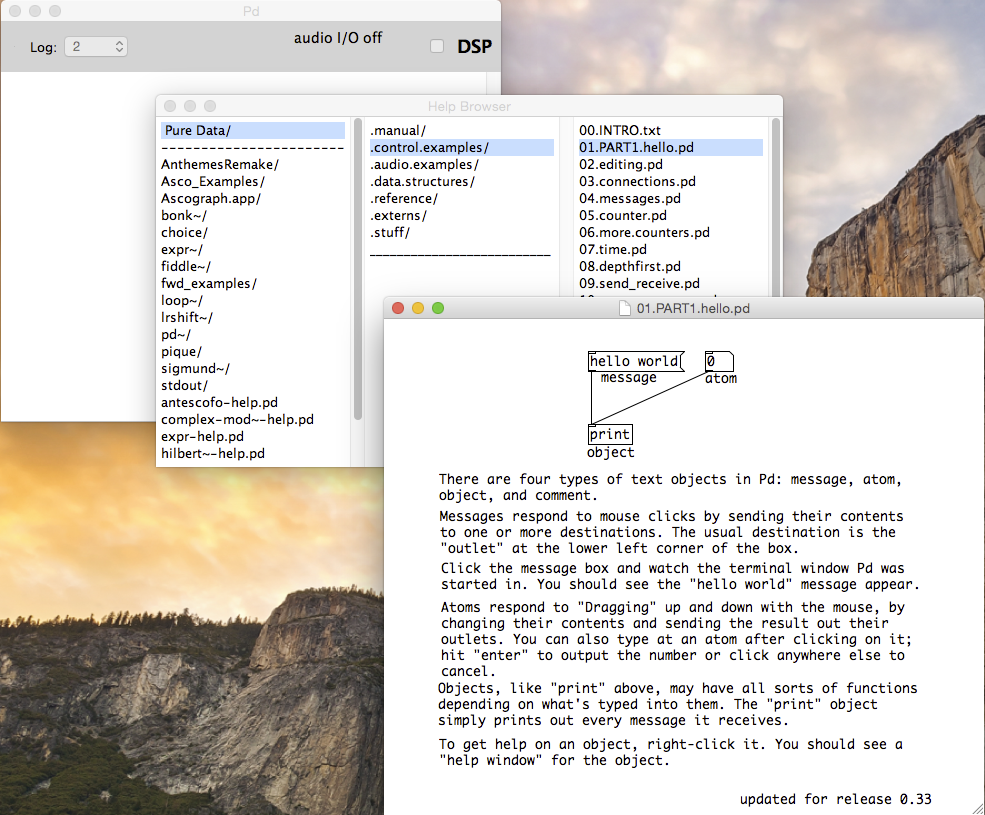
\includegraphics[scale=0.4]{fig/pd-help-browser.png}
    \caption{Pure Data Help Browser}
    \label{fig:pd-help-browser}
\end{figure}


\subsection{Antescofo}

``Antescofo is a modular polyphonic Score Following system as well as a
Synchronous Programming language for musical composition. The module allows
for automatic recognition of music score position and tempo from a realtime
audio Stream coming from performer(s), making it possible to synchronize an
instrumental performance with computer realized elements. The synchronous
language within Antescofo allows flexible writing of time and interaction in
computer music.''~\cite{website:antescofo}

Material: technical documentation, demo patch, alle meine events
Source for specific answers: the web, Antescofo user group

\subsection{Logic Pro}

Logic Pro~\cite{website:logic} is a professional MIDI and audio recoding
software for OSX. It supports all features required for the project, i.e.,
processing multiple audio tracks together with real-time MIDI instruments for
synthesizing sounds while playing with Antescofo and recording the piece in
high quality.  Note that there are many similar tools, including free and open
source software, that would do the trick. Nevertheless, we choose Logic Pro
for one reason. One of the students had prior knowledge with Logic Pro.


Material: examples of multi-track multi-instrument projects showing
the non-linear production process of software sequencers. Once you know
the work flow of multi-track audio production, all tools suddenly look similar.
Source for specific answers: the web

\subsection{iMovie}

Material: 
Source for specific answers: the web


Note that similar to Logic Pro, there are plenty of alternative software
tools to do the job. Again, one student had prior knowledge in working
with iMovie. 


\section{Description of the Tasks}

\subsection{Setting up the team}

Making the students getting to know each other. First Task: ``Talk about music!''

\subsection{Getting started with Pure Data}

%using the help browser. add screen shot. give example

Antescofo is implemented in - and controlled through - Pure Data.
Installing Pure Data is as simple as installing any OSX application. Details can be found
on the Pure Data website and are not repeated here\footnote{https://puredata.info/downloads}.

A Pure Data application is called a patch. A patch has a graphical Pure Data window



\begin{figure}[ht]
    \centering
    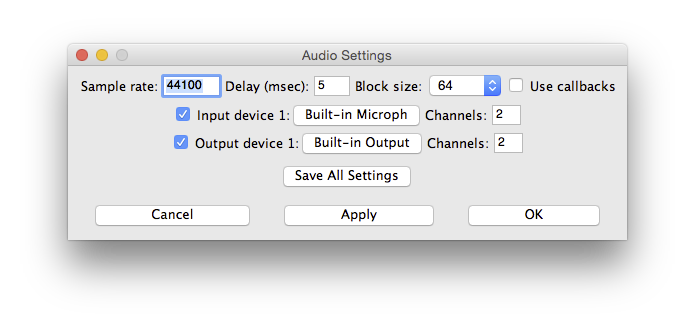
\includegraphics[scale=0.4]{fig/pd-audio.png}
    \caption{Pure Data Audio Settings}
    \label{fig:pd-audio}
\end{figure}


\begin{figure}[ht]
    \centering
    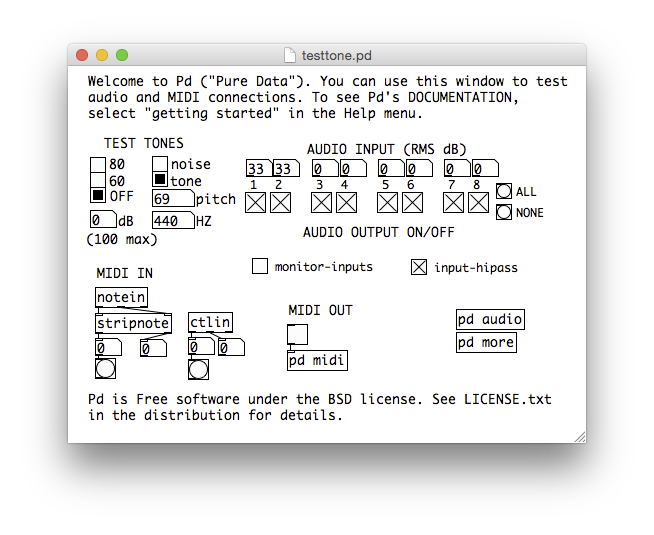
\includegraphics[scale=0.4]{fig/pd-test.png}
    \caption{Pure Data Audio Test Patch}
    \label{fig:pd-test}
\end{figure}



\subsection{Implement your first Pure Data Patch}

Do something nice with Pure Data


\subsection{Getting started with Antescofo}

%audio setup. events and actions. alle meine events

Hand out the manual.

Understand events and actions.





\section{Time Table}

The time frame for the project is approximately 2 weeks, 6 hours per day, or
60 hours. Note that the time table is heavily affected by the students' prior
knowledge in programming. Table REFERENCE gives a brief overview of the
suggested time required for each individual project task.






4 weeks, preparation classes, prerequisites




\section{Acknowledgments}

The project was supported by the Austrian Research Promotion Agency (FFG) FFG-Nr 851846, but it
was only possible because of the students: Matthäus Mayr, Amrita Newton, Hannah Schmidbauer, and
Leonard Trommler. Thanks a lot!

\bibliographystyle{IEEEtran}
\bibliography{sources} 


\end{document}


